\clearpage
\section{Implementácia}\label{sec:programming}

Aplikácia pozostáva z dvoch častí a to \textbf{časť umelej inteligencie} a \textbf{hra}.
V časti umelej inteligencie sa vytvára a trénuje umelá neurónová sieť, v hernej časti sa dá hra ovládať pomocou
ovládača od hernej konzoly Xbox a zobrazená je v prostredí \emph{Cave}.

\subsection{Unity}\label{subsec:unity}
Samotná ovládacia časť (hra) je vytvorená v prostredí Unity verzie 2019.2.17f1.
Unity je framework (alebo engine) pre vytváranie 2D alebo 3D hier/simulácii/modelov a v súčasnosti je považovaný za
jeden z najlepších a najpoužívanejších nástrojov pre vývoj 2D a 3D aplikácii.
V jadre Unity sa nachádza mnoho už vyvinutých modulov (ako je napr. gravitácia pre 3D objekty, kamera pre zobrazovanie
z pohľadu hráča, \dots).
Ďalšie súčasti sa dajú vyvinúť s použitím aplikácie Unity Editor, kde sa dajú buď zložiť z existujúcich súčastí
alebo doprogramovať v jazyku C\#, s ktorým Unity pracuje.
Projekt pozostáva z niekoľkých modulov:

\textbf{Scény} sú v rámci unity kontajnery pre herné objekty (napr. 3D model) v rámci jedného logického celku.
Scéna je v klasických hrách ekvivalentom levelu alebo prostredia, v ktorom sa hráč nachádza.
V hre sa nachádzajú dve scény: scéna pre hlavné menu a scéna pre hraciu plochu.

Ďalšou dôležitou časťou sú \textbf{vopred pripravené súbory} (angl. a ďalej len \emph{prefabs}), čo sú v podstate herné
objekty, ktoré sú zložené z už existujúcich herných objektov pre účely znovupoužitia.
Vytvorené sú prefabs pre tlačidlo v menu, posuvník v menu (pre výber napr. veľkosti hracieho priestoru), oddeľovač
buniek v hracom priestore, bunku v hracom priestore a znaky \textbf{X} a \textbf{O} vytvorené pre 3D priestor.

\textbf{Skripty} sú funkčnou časťou celej aplikácie.
Unity má veľké množstvo skriptov už vopred pripravených, no pre konkrétne využitie je vo väčšine prípadov nutné si
vytvoriť vlastné skripty.
V hre je ich použitých 10:
\begin{enumerate}
    \item \emph{BoardOperations} obsahuje operácie pre hraciu plochu ako napr. nájdenie víťazného hráča
    \item \emph{ButtonController} ovláda všeobecne tlačidlá v hlavnom menu
    \item \emph{Cell} skript priradený pre jednu bunku v hracej ploche
    \item \emph{Focusable} akýkoľvek prvok v hlavnom menu, na ktorý sa dá "pozrieť"
    \item \emph{GameController} ovláda celý proces v rámci hry
    \item \emph{Grid} je kontajner pre herný priestor
    \item \emph{HudController} ovláda prvky v menu
    \item \emph{PlayerController} obsahuje funkcie pre pohyb hracieho priestoru v zornom poli hráča
    \item \emph{SliderItemController} - posuvník v menu
    \item \emph{BuildScript} spúšťa zostavenie spustiteľného súboru pre platformu Windows
\end{enumerate}

V ostatných súboroch sa nachádzajú stiahnuté \textbf{3D súbory} a \textbf{knižnice}, \textbf{materiály} pre 3D objekty
a \textbf{font} pre písmo v menu.
Zvyšné súbory sú generované vývojovým prostredím.

\begin{figure}[H]
    \centering
    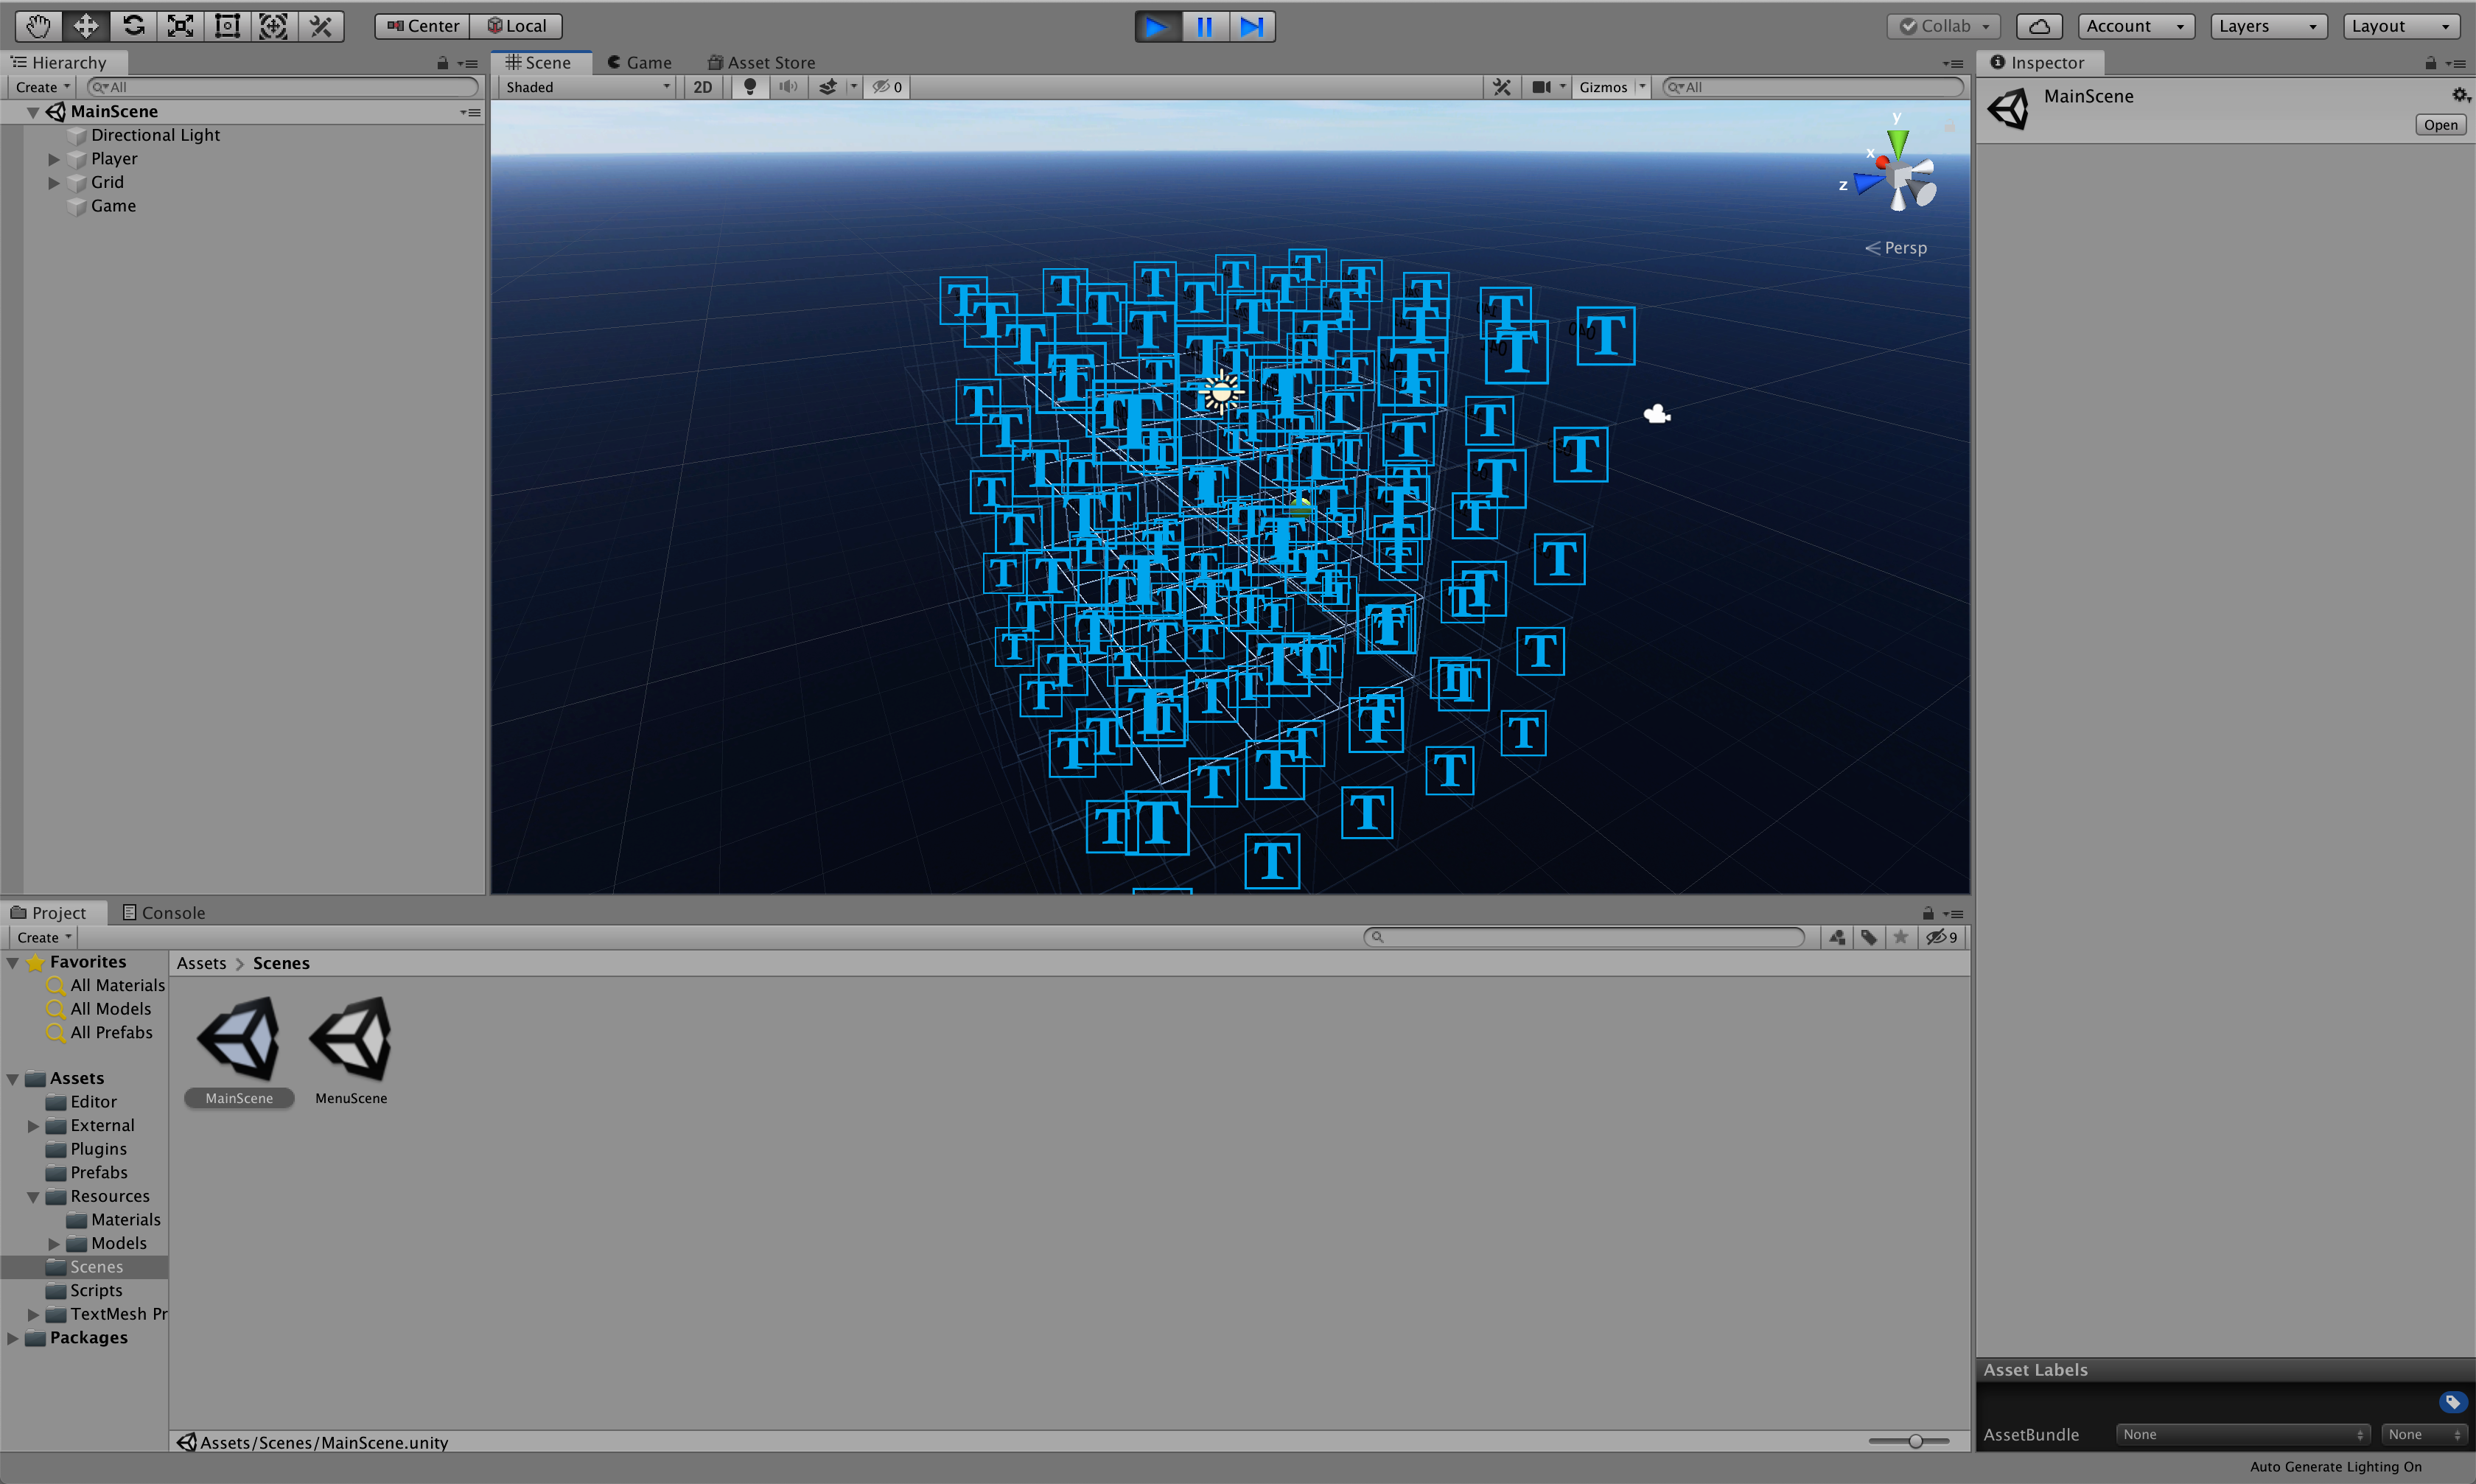
\includegraphics[width=0.8\textwidth]{images/unity.png}
    \caption{Prostredie unity}
\end{figure}\label{figure:unity}

V unity sú vstupy mapované do tzv. osí, čo dovoľuje použitie viacerých zariadení pričom pre všetky zariadenia existuje
len jeden kód.
Napr. pre použitie joystick-u a tlačidiel pre šípky vpravo alebo vľavo sa použije os s názvom \enquote{Horizontal},
ktorej hodnota je -1 v prípade, že užívateľ posunie joystick vľavo, resp. stlačí ľavú šípku a hodnota je 1 v prípade,
že užívateľ posunie joystick vpravo, resp. stlačí pravú šípku.
Pomocou týchto osí je možná napr. navigácia v hlavnom menu alebo otáčanie hracieho priestoru.

\subsubsection{Prostredie Cave}
Cave prostredie je také, ktoré zobrazuje obraz na štyroch plochách súčasne.
Ak pozorovateľ stojí priamo, tak jedno plátno je pred ním, ďalšie sú vpravo a vľavo kolmé na plátno pred ním a posledné
je plátno pri nohách pozorovateľa.
Projektory sú umiestnené nad celým týmto systémom a navyše sa celý obraz zobrazuje upravený pre 3D okuliare.
Systém je zobrazený na obrázku nižšie.
Unity pracuje najmä s prostredím \textbf{KAVE} (skr. Kinect Cave) a teda už z názvu vyplýva, že celý systém ovládania
je založený na Microsoft Xbox Kinect a preto aj ovládanie prebieha pomocou ovládača k zariadeniu Xbox.

\begin{figure}[H]
    \centering
    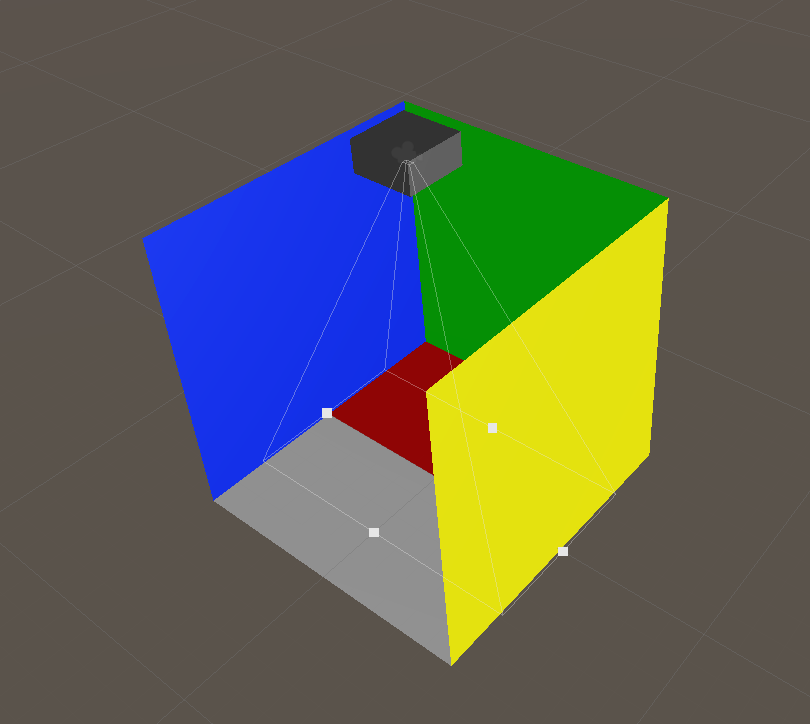
\includegraphics[width=0.4\textwidth]{images/kave.png}
    \caption{Prostredie Cave}
\end{figure}

V súvislosti s karanténou spojenou so šíriacim sa ochorením Covid-19 nebolo možné dokončiť aplikáciu v prostredí Cave,
no je plne funkčná ako desktopová aplikácia s možnosťou behu na akejkoľvek platforme (Windows, MacOS, resp. OSX aj
Linux).

\subsection{Vývojové prostriedky pre umelú inteligenciu}\label{subsec:dev-tools-for-ai}

Oba algoritmy umelej inteligencie (minimax a umelá neurónová sieť) boli implementované v jazyku Python verzie 3.7.

\subsubsection{Minimax}

Pretože samotný pseudokód algoritmu minimax je jednoduchý, aj jeho implementácia je triviálna:
\begin{figure}[H]
    \centering
    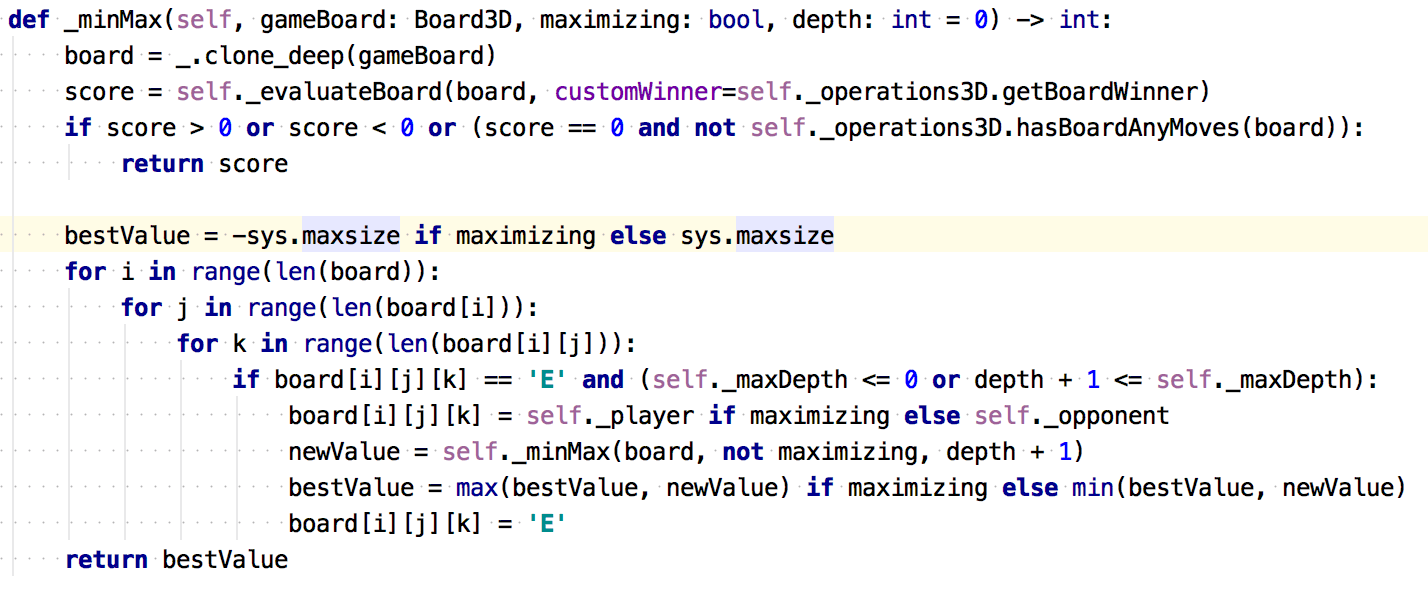
\includegraphics[width=0.8\textwidth]{images/impl-minimax.jpg}
    \caption{Implementácia algoritmu minimax}
\end{figure}\label{figure:minimax-impl}

\subsubsection{Umelá neurónová sieť}

Pre implementáciu algoritmov umelej inteligencie, existuje knižnica \emph{Tensorflow}\cite{tensorflow} od spoločnosti
Google.
Táto knižnica okrem umelých neurónových sietí ponúka aj možnosti pre implementáciu pre mnohé iné algoritmy týkajúce sa
strojového učenia.
Pre potreby umelých neurónových sietí bola vyvinutá knižnica \emph{Keras}\cite{keras}, ktorú vyvíja viac vývojárov
(no za hlavného autora sa považuje Google).
Keras umožňuje definovať štruktúru neurónovej siete, Tensorflow túto sieť natrénuje.
Okrem implementácie tried a štruktúr programu sú dôležité práve dve časti a to štruktúra umelej neurónovej siete a
trénovanie umelej neurónovej siete.

Model bol vytvorený na základe návrhu v \autoref{subsec:algo-ann} a jeho parametre boli nastavené na základe
štruktúr použitých v programe.
Jedná sa teda o $3r^d$ vstupov (inputs), kde $d=3$ pretože daná sieť je implementovaná v rámci 3D priestoru a $r$ je
rovné veľkosti poľa \emph{board}.
Pole board je síce trojrozmerné, no keďže veľkosť je rovnaká v každom rozmere (kocka), stačí použiť veľkosť hlavnej
štruktúry.
Jediná skrytá vrstva má veľkosť $r^d$ a výstup, aj keď je v \autoref{subsec:algo-ann} uvedené, že na výstupe je len
jedno číslo (index s najväčšou pravdepodobnosťou výhry), knižnica Tensorflow vyžaduje aby týchto výstupov bolo $r^d$.
Dôvodom tohto prístupu je fakt, že z technického hľadiska sa jedná o \emph{klasifikáciu} (zaradenie vstupu k jednému z
výstupov).
Knižnica z $r^d$ možností pohybu hráča rozhodne o tom, ktoré políčko má pre hráča najvyššiu pravdepodobnosť výhry
pomocou tzv. \emph{one-hot array}.
Je to vektor (pole) $s_i$, ktory má $r^d$ prvkov, $\forall i : i\neq k s_i=0$ a $s_k=1$, kde $k$ označuje index
políčka s najpravdepodobnejším víťazstvom.
Napr. pre $r=3$, $d=3$ a $k=4$ pole vyzerá nasledovne:
\begin{equation}
    s = <0, 0, 0, 1, 0, 0, 0, 0, 0>
\end{equation}

Model je vytvorený ako sekvenčný, čo znamená, že sieť je dopredná (signál sa šíri iba smerom od vstupnej vrstvy k
výstupnej).
Všetky vrstvy v sieti sú označené ako \emph{dense}, čo vyjadruje, že všetky neuróny $i$-tej vrstvy sú prepojené z sú
prepojené so všetkými neurónmi vrstvy $i+1$.
Všetky neuróny vstupnej a skrytej vrstvy sú aktivované pomocou funkcie \emph{ReLu} (\emph{activation=relu}), posledná
vrstva obsahuje neuróny aktivované pomocou funkcie \emph{SoftMax} (\emph{activation=softmax}).
Posledná vrstva vyžaduje túto aktivačnú funkciu, pretože výstupom z nej je klasifikácia.
Model je kompilovaný s účelovou funkciou \emph{kategorická krížová entropia} (loss=categorical\_crossentropy).
Pri riešení minimalizačnej úlohy v rámci umelej neurónovej siete je využitý \emph{RMSProp optimizer} založený na
stochastickej gradientovej metóde (\emph{optimizer=rmsprop}).
Ukazovateľ optimality je presnosť v zaradení do jednotlivých kategórií (\emph{metrics=[acc]} - možnosť vyplniť viac
ukazovateľov).

\begin{figure}[H]
    \centering
    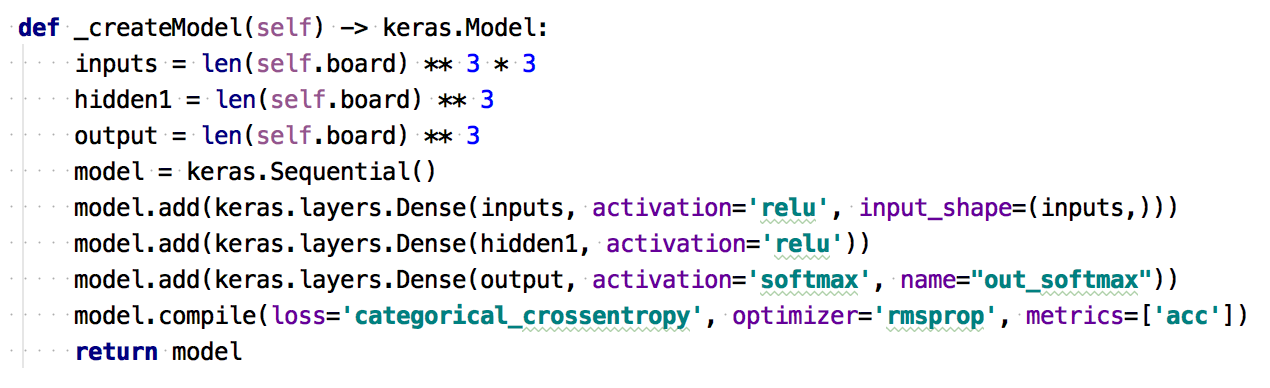
\includegraphics[width=0.8\textwidth]{images/impl-ann-model.jpg}
    \caption{Implementácia štruktúry umelej neurónovej siete}
\end{figure}\label{figure:ann-model-impl}

Pre potreby trénovania je nutné pripraviť vzorku dát pre umelú neurónovú sieť.
Tieto dáta sa získavajú simulovaním náhodných hier a sú rozdelené na dáta pre hráča a dáta pre oponenta.
Dáta pre oponenta sa využívajú len pri experimentoch.
Obe tieto skupiny sú rozdelené na vstupnú časť a výstupnú časť, pričom sú rozdelené ešte na trénovaciu a testovaciu časť
v pomere 4:1 (4 trénovacie vzorky na 1 testovaciu).

\begin{figure}[H]
    \centering
    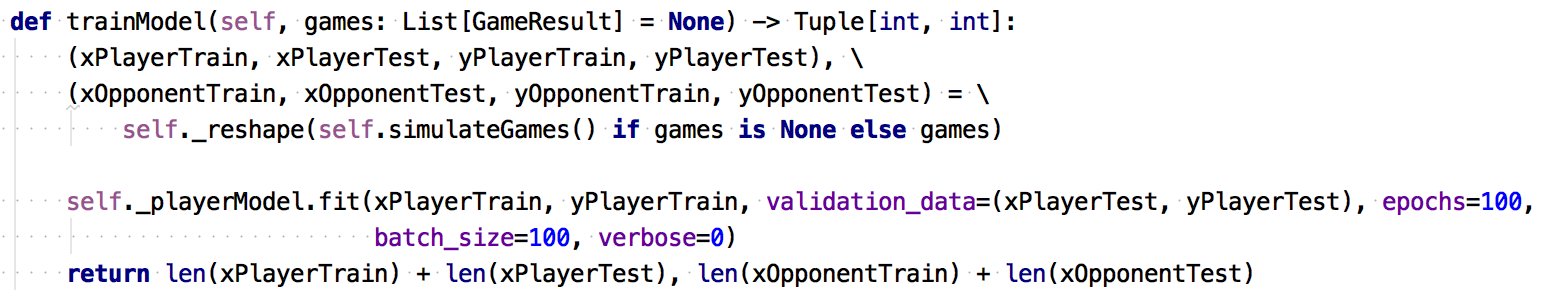
\includegraphics[width=0.8\textwidth]{images/impl-ann-train.jpg}
    \caption{Implementácia trénovania umelej neurónovej siete}
\end{figure}\label{figure:ann-train-impl}

\subsection{Prepojenie umelej inteligencie s prostredím}\label{subsec:connection}

Aby sa mohli natrénované modely využiť pre praktické použitie (v hre) je možné tieto modely uložiť na disk.
Ukladanie prebieha jednoducho zavolaním metódy \emph{save} a \emph{save\_weights} nad natrénovaným modelom a definovaním
cesty pre uložené súbory.
Následne je potrebné uložiť ešte aj celú reláciu trénovania (pomocou \emph{freeze\_session}) a nakoniec zapísať celú
štruktúru ako graf s použitím \emph{write\_graph}.
Tento graf sa do súboru uloží ako binárny súbor.
\begin{figure}[H]
    \centering
    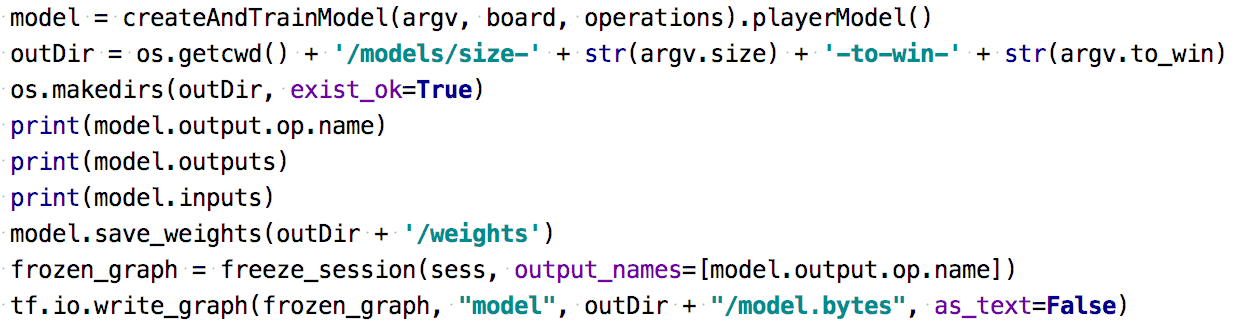
\includegraphics[width=0.8\textwidth]{images/impl-ann-save.png}
    \caption{Implementácia ukladania ANN na disk}
\end{figure}\label{figure:ann-save-impl}
Modely sa ukladajú do samostatných priečinkov pomenovaných nasledovne: \enquote{size-$r$-to-win-$w$}.
Pre použitie tejto uloženej štruktúry je možné využiť knižnicu \emph{TensorflowSharp}, ktorá je vyvinutá pre C\# a ktorá
poskytuje viac-menej tie isté možnosti ako Tensorflow pre python.
V aplikácii je použitá pre načítanie modelov z disku a ich použitie v samotnej hre.
\begin{figure}[H]
    \centering
    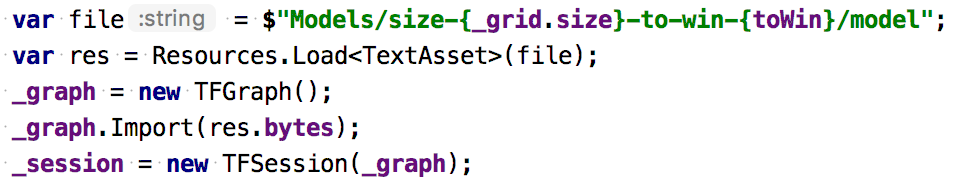
\includegraphics[width=0.8\textwidth]{images/impl-ann-load.png}
    \caption{Implementácia načítania ANN z disku}
\end{figure}\label{figure:ann-load-impl}
\begin{figure}[H]
    \centering
    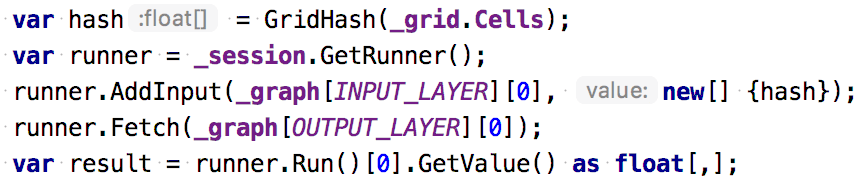
\includegraphics[width=0.8\textwidth]{images/impl-ann-usage.png}
    \caption{Implementácia použitia ANN v aplikácii}
\end{figure}\label{figure:ann-usage-impl}

\subsection{Cloud computing}\label{subsec:ci}

Za účelom automatizácie a zrýchlenia zostavenia bol nastavený aj continuous deployment (súvislé nahrávanie, ďalej len
"CD") na \emph{GitLab-CI}.
Toto nastavenie umožňuje spustiť trénovanie umelej neurónovej siete a zostavenie aplikácie priamo na serveroch,
Konkrétne sa jedná o servery od spoločnosti \emph{Amazon} v rámci divízie \emph{Amazon web services}.
Na trénovanie ANN sa použila inštancia Linuxového serveru optimalizovaného pre lepší výkon operačnej pamäte.
Pre zostavenie unity aplikácie (s využitím natrénovanej umelej neurónovej siete) bola použitá inštancia Windows
serveru s predinštalovanou aplikáciou Unity.
\begin{figure}[H]
    \centering
    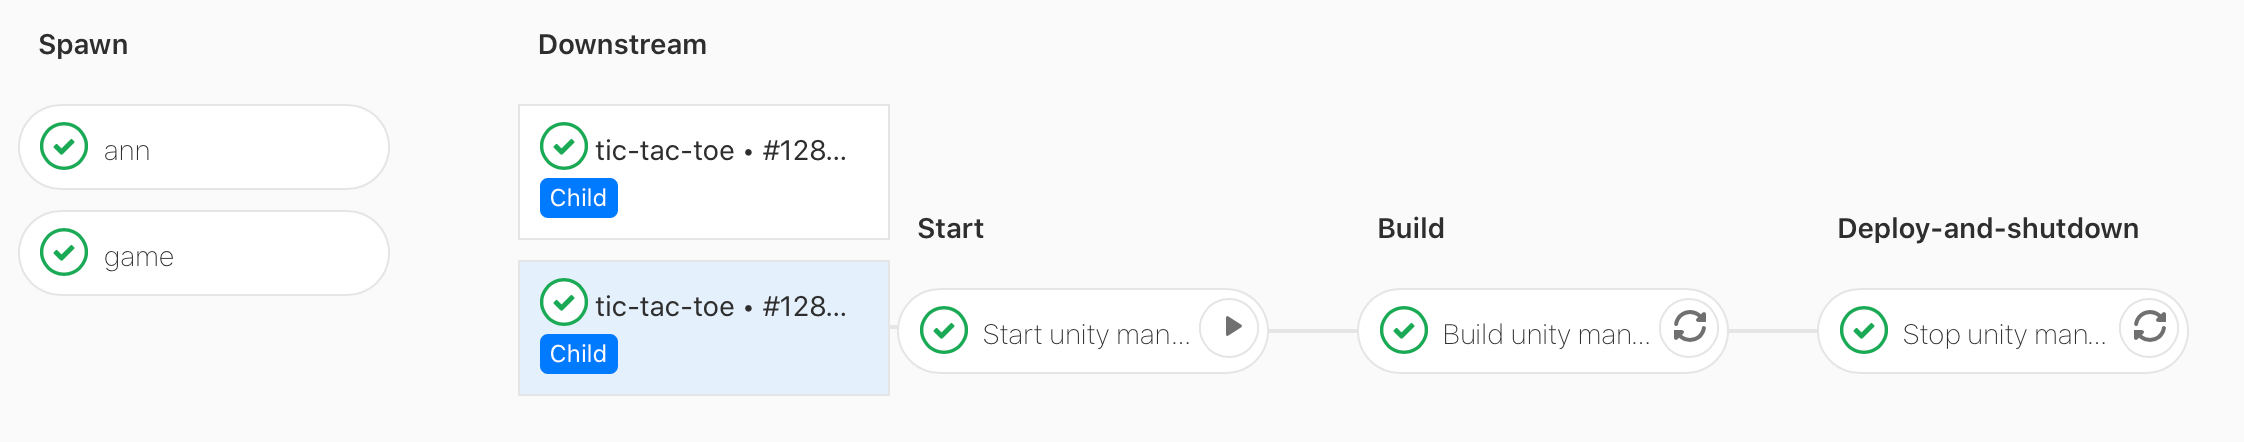
\includegraphics[width=1\textwidth]{images/impl-cd.png}
    \caption{Zobrazenie zotavenia aplikácie v rámci continuous deployment}
\end{figure}\label{figure:cd}

\subsection{Príručky}\label{subsec:helpers}
\subsubsection{Umelá inteligencia}
Ako bolo vyššie spomenuté, časť aplikácie, ktorá je zameraná na umelú inteligenciu, je implementovaná v jazyku python.
Interakcia s touto časťou je vykonávaná prostredníctvom rozhrania príkazového riadku (skr. CLI, angl. command line
interface), pričom pre použitie je potrebné mať nainštalovaný interpreter jazyka python.
Znamená to, že program nie je skompilovaný do jedného binárneho balíku (bundle) a je nutné pracovať priamo so zdrojovým
kódom.
Python verzie 3.7.4 a pip 19.0.3 (čo je nástroj pre správu závislostí projektu) boli použité pre vývoj aplikácie.
Pred začatím používania je nutné nainštalovať všetky závislosti zo súboru \emph{requirements.txt}.
Tento súbor obsahuje informácie o balíčkoch a ich konkrétnych verziách použitých v projekte.
Pre odstránenie potenciálneho konfliktu už nainštalovanej verzie je odporúčané vytvoriť si tzv. virtuálne prostredie
(angl. virtual environment).
Jedná sa o vytvorenie priečinku, v ktorom sú obsiahnuté všetky informácie (interpreter, balíčky) týkajúce sa daných
požiadaviek projektu (najmä závislosti).
Takýmto spôsobom sa vytvorí izolované prostredie pre projekt, ktoré je nezávislé od globálneho.
Použitie aplikácie je napr.: \shellcmd{python ./src/\_\_main\_\_.py game}.

Predpis použitia je \shellcmd{python ./src/\_\_main\_\_.py [task] [parameters]} a aplikácia prijíma nasledovné
argumenty:
\begin{itemize}
    \item \shellcmd{task}: (slovensky \enquote{úloha}) vyjadruje analogicky úlohu, ktorá sa má vykonať.
    Možný je výber z nasledujúcich:
    \begin{itemize}
        \item \shellcmd{ann}: spustenie simulácie s trénovaním umelej neurónovej siete
        \item \shellcmd{minmax}: spustenie simulácie s využitím algoritmu minimax
        \item \shellcmd{analyze}: spustenie experimentov s rôznymi plochami
        \item \shellcmd{game}: spustenie experimentov s rôznymi modelmi
        \item \shellcmd{playground}: z názvu vyplýva, že je na programátorovi, čo sa spustí v rámci tohto príkazu, pričom sú
        dostupné všetky potrebné náležitosti, ktoré majú dostupné aj iné úlohy
        \item \shellcmd{store-ann}: natrénovanie a uloženie neurónovej siete
    \end{itemize}
    \item \shellcmd{\-\-size=[number]}: rozmer hracej plochy (resp. hracieho priestoru); ekvivalent $r$
    \item \shellcmd{\-\-to-win=[number]}: počet rovnakých, za sebou idúcich znakov potrebných pre výhru; ekvivalent $w$
    \item \shellcmd{\-\-dimension=[number]}: dimenzia (2 alebo 3); ekvivalent $d$
    \item \shellcmd{\-\-player=[X,O]}: preferovaný (cieľový) hráč
    \item \shellcmd{\-\-simulations=[number]}: počet simulácii hier (resp. veľkosť trénovacej množiny)
    \item \shellcmd{\-\-validations=[number]}: počet validácii (slúži pre získanie reálnych štatistík)
    \item \shellcmd{\-\-max-depth=[number]}: maximálna veľkosť vyhľadávacieho stromu pri algoritme \emph{minimax};
    ekvivalent $l$
    \item \shellcmd{\-\-ann-model=[adaptive,large]}: zvolený model \emph{umelej neurónovej siete}
    \begin{itemize}
        \item \shellcmd{adaptive} je model popísaný v \autoref{subsec:algo-ann}
        \item \shellcmd{large} je model použitý pri experimentoch, popísaný v \autoref{subsec:experiments-board}
    \end{itemize}
\end{itemize}

\subsubsection{Hra}

\paragraph{Programátorská príručka}
Unity verzie 2019.2.17f1 bolo použité pri vývoji užívateľskej časti aplikácie.
V rámci projektov unity je odporúčané držať sa verzie, v ktorej je projekt vyvíjaný, pretože pri zložitejších
štruktúrach môže dôjsť ku konfliktom.
Pre otvorenie projektu vo vývojovom prostredí je nutné mať nainštalovanú túto verziu unity a aplikáciu
\enquote{unity editor}.
V tomto programe je možné upravovať vizuálnu stránku aplikácie, vytvárať moduly a meniť väzby medzi nimi.
Pre úpravu kódu v rámci jazyka C\# je možné použiť akékoľvek vývojové prostredie (skr. IDE, angl. integrated development
environment), ktoré podporuje tento jazyk.
Medzi najpoužívanejšie patria \emph{Microsoft Visual Studio} alebo \emph{JetBrains Rider}, v ktorom bola aplikácia
vyvíjaná.
Aplikáciu je možné skompilovať dvoma spôsobmi:
\begin{enumerate}
    \item odporúčaným spôsobom v danom IDE
    \item pomocou príkazového riadku.
    Ako príklad je možné uviesť kompilovanie v OS Windows:
    \shellcmd{"c:{\textbackslash}Program Files{\textbackslash}Unity{\textbackslash}Hub{\textbackslash}Editor{\textbackslash}2019.2.17f1{\textbackslash}Editor{\textbackslash}Unity.exe"\\ \-batchmode \-nographics \-executeMethod BuildScript.PerformBuild \-quit \-projectPath game \-logFile \-}
    Tento konkrétny zápis je použitý aj pri zostavení aplikácie v GitLab-CI .
\end{enumerate}

\paragraph{Používateľská príručka}
Zostavený program je pripravený pre použitie aj na klasickom desktopovom počítači aj v prostredí Cave.
Pri zapnutí programu sa zobrazí hlavné menu, kde sú dve možnosti: začať hru a ukončiť program (oba s anglickými
názvami).
Navigácia v menu je vykonávaná pomocou vertikálnej osi.
Zvolením možnosti ukončiť program sa aplikácia vypne, po zvolení možnosti začať hru je zobrazené ďalšie menu, kde si
používateľ volí parametre hry.
Konkrétne ide o veľkosť hracieho priestoru (3-8), počet za sebou idúcich znakov potrebných pre výhru a znak hráča, s
ktorým chce užívateľ hrať.
Parametre sa volia využitím horizontálnej osi.
Po vyplnení všetkých potrebných parametrov sa hra spustí.
Pomocou oboch osí je možné otáčať hrací priestor, pričom najbližšie políčko, na ktoré sa \enquote{pozerá kamera} je
vyznačené zelenou guľou.
V hre sa navyše využívajú navyše ešte 3 osi pre akčné tlačidlá:
\begin{enumerate}
    \item priblíženie v rámci hracieho priestoru
    \item oddialenie v rámci hracieho priestoru
    \item priradenie vlastného znaku na označené políčko
\end{enumerate}
Po priradení znaku sa automaticky vyplní aj jedno políčko protihráča, ktoré vyberie algoritmus umelej inteligencie.
V prípade, že jeden z hráčov vyhrá alebo nastane remíza s tým, že všetky políčka sú už obsadené, vypíše sa na obrazovku
informácia o stave hry a po 7 sekundách je uskutočnený návrat do hlavného menu.

